\iffalse
https://edoc.sub.uni-hamburg.de/hcu/volltexte/2017/370/pdf/Ebert_Kirsten.pdf Anfang
\fi
%synonym handelsmodelle

\begin{folding} % Einleitung

Im folgendem werde ich Verkäufer aller Art ähnlich wie im Buch "Das E-Commerce Buch: Marktanalysen - Geschäftsmodelle - Strategien" unterteilen: in Online-Marktplätze, Online-Händler, Kataloversender, stationäre Händler und Hersteller\cite[S. 15ff]{Graf}. Dabei sind Online-Marktplätze eine Art Online-Vermittler zwischen Kunden und Verkäufer, Online-Händler bieten dagegen nur eigene, meist sehr spezialisierten Sortimente an. Kataloversender verhalten sich ähnlich: sie versenden ihr Sortiment direkt an Kunden. Stationäre Händler verkaufen im Gegensatz zu den genannten Vertreibsstrukturen in Fillialen und sind mit Kataloghändlern am stärksten von den Änderungen der letzten Jahrzenten betroffen. Während sich die genannten Unternehmensarten meistens am Ende der Verkaufskette befinden, stehen Hersteller am Anfang: sie stellen Güter her und sind dementsprechend, insofern sie nicht selber verkaufen, auf weitere Unternehmen für Verkauf und Vermarktung angewiesen(ebd.). %vor und -nachteile?; beispielsunternehmen

\end{folding}

\begin{folding} % KATALOGHÄNDLER

Kataloghändler sind die größten Verlierer der letzten Jahrzehnte: mit der Entwicklung des Onlinehandels ist ab 2002 schon ein Rückgang der Nachfrage zu spüren – einige eröffnen eigene Online-Shops\cite[S. 24f]{Graf}, jedoch oft mit wenig Erfolg\cite[S. 38]{Graf}. 2015 sind Katalogversender fast ausschließlich verschwunden oder zu Online- und Einzelhandel konvertiert, da sie kaum einen Mehrwert im Vergleich zum klassisschen Onlinehandel bieten\cite[S. 47]{Graf}. So prognostiziert beispielsweise 2012 IFH Retail Consultants einen einen sinkenden Anteil des Online-Umsatzes von 24.9\% zu 23.9\% in den folgenden 2 Jahren\cite[S. 20]{evilcom}. Tatsächlich fiel der Anteil aber ganze 4.6\% - knapp das fünffache des erwarteten Wertes\cite{statista-vertriebsformen}. %Zusätzlich wird ein Umsatzanteil von 16.6\% für 2019 vorrausgesagt. ::: zu viel wirtschaft

\end{folding}

\begin{folding} % STATIONÄR
    % nitt S 54 these, dass einzelhandel zurückkommt
Der stationäre Handel ist durch die steigende Relevanz des Onlinehandels auch weniger gefragt denn je und versucht mit strukturellen Änderungen dagegen anzukämpfen. Einige Einzelhändler eröffenen paralel zu ihrem Geschäft einen Online-Shop, andere bieten die Möglichkeit, Waren online in den Laden zu bestellen und diese dort anzuholen – sogenanntes "Multichannel-Marketing", das Ansprechen der Kunden über mehrere Wege\cite[S. 34f]{Graf}. Jedoch fahren die neuen Strkturen nur wenig Erfolge ein – so erhöhen sie zwar die Onlinepräsenz, bieten jedoch nur einen geringen Mehrwert im Vergleich zu den bekannten Onlineriesen wie Amazon\cite[S. 34f]{Graf}. 
Schließlich stellt sich die Frage, welche Vorteile der stationäre Handel noch bieten kann, um die im Vergleich zum Onlinehandel deutlich höheren Preise zu rechtfertigen - denn pure Onlinehändler haben deutlich dünnere Kostenstrukturen\cite[S. 14]{evilcom}. So müssen sie etwa keine Miete für Geschäfte zahlen und kommen mit deutlich weniger Angestellten aus, folglich weniger Kosten.

Einer dieser Vorteile ist in der Theorie der soziale Aspekt des Einkaufens, der laut Nitt-Drießelmann vorallem für über-50-Jährige, die über viel Freizeit verfügen, eine immer größer werdende Rolle spielen wird\cite[S. 43f]{Nitt}:
\begin{quote}
"Als Mittel gegen Vereinsamung und Anonymisierung im Alltag wird die soziale Komponente beim Einkaufen [...] zunehmend an Bedeutung gewinnen."\cite[S. 43]{Nitt}
\end{quote} 
So soll in Zukunft der Wunsch nach Begegnungen mit bekannten Personen und Beratung zunehmen und die Zusammensetzung von sozialen Kontakten eine immer wichtigere Rolle spielen(ebd.).
Außerdem müssen stationäre Händler stärker auf die geänderten Wünsche an Sie von Konsumenten eingehen. Beispielsweise wollen Sie einen bequemen Einkauf mit langen Öffnungszeiten, eine übersichtliche Warenpräsentation sowie eine möglichst große Produktauswahl auf einer so kleinen Verkaufsfläche wie möglich\cite[S. 61]{Nitt}.

Zu dem kommt, dass in Deutschland bedeutende demografische Änderungen bevorstehen: so schrumpft und altert die Gesamtbevölkerung, folglich muss der stationäre Handel sich auf einen zusätzlichen Nachfragerückgang einstellen sowie die Bedürfnisse von Senioren stärker beachten - insbesondere auf dem Land, denn in Metropolen soll das Durchschnittsalter nahezu konstant bleiben\cite[S. 32ff]{Nitt}. Diese Chance kann er aber nur nutzen, indem er stärker auf die Bedürfnisse der älteren Bevölkerung, die 2050 etwa 59\% der Kaufkraft ausmachen soll, eingeht\cite[S. 64]{Nitt}. So kaufen Sie oft Qualitätsprodukte in den Bereichen Gesundheit, Wohnen und Energie - jedoch kaum langlebige Konsumgüter, da Sie diese schon besitzen; zusätzlich sehen sie kein Problem damit, für kompetente Beratung mehr zu bezahlen\cite[S. 41f]{Nitt}. Folglich muss der stationäre Handel die Produktauswahl sowie Erreichbarkeit und Übersichtlichkeit auf die alternde Bevölkerung anpassen, um die beste Kaufoption für Sie zu bleiben\cite[S. 64]{Nitt}.

Obwohl in Zukunft die Bevölkerung Deutschlands schrumpfen wird, ist eine erhöhte Anzahl von Haushalten zu erwarten - durch eine "Zerstreuung" der Haushaltsstruktur. So soll es 2030 1.8 Mio. weniger Mehrpersonenhaushalte geben, dafür aber 1.4 Mio. Einpersonen- sowie 1.6 Mio. Zweipersonenhaushalte mehr als 2010\cite[S. 35]{Nitt}, was zu einer automatischen Erhöhung der Wochnfläche pro Person führt. So werden Haushaltsprodukt- und Möbelverkäufer in den nächsten Jahren weniger von Insolvenzen betroffen sein wie Unternehmen anderer Branchen.

Zusätzlich gibt es beim stationären Handel Produkte, die nicht oder nur schwer durch andere Vertriebswege abzudecken sind, wie etwa beratungsintensive Waren
%https://de.statista.com/statistik/daten/studie/201914/umfrage/einkaufsverhalten-im-onlinehandel-vs-einzelhandel-nach-produktgruppen/

%"feeling" des produktes

%handwerker: kaum durch online ersetzbar, allerdings ist ein pur stationärer handwerkerbetrieb auch nicht zukunftsfähig.

\end{folding}

\begin{folding} % ONLINE

Die Onlinehändler und -marktplätze sind die Gewinner der letzten 20 Jahre – die Verkäufswerte wuchsen ab der Jahrtausendwende konstant an und stellen in vielen Branchen für andere Vertriebsstrukturen eine ernst zu nehmende Konkurrenz dar\cite{wolf}. Vorerst wechseln Konsumenten von Katalogen, ab 2010 auch viele Nutzer anderer Verkaufswege, da das Kaufen online fast immer einen Preisvorteil bietet\cite[S. 31]{Graf}.
\begin{figure}[h]
    \begin{center}
        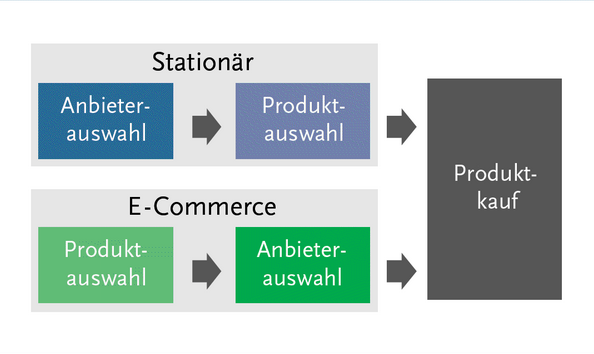
\includegraphics[width=8cm]{media/Fabian-konsumwandel.png}
        \caption{Kaufprozess im Vergleich – Stationär und E-Commerce}
        \label{konsumwandel}
        \bildquelle Björn Schäfers, Social Shopping für Mode, Wohnen und Lifestyle am Beipiel Smatch.com in Web-Exzellenz im E-Commerce, Gabler, S. 313 %lieber quelle e com buch???
    \end{center}
\end{figure} 
Außerdem hat sich unter Nutzern des Onlinehandels ein neues Konsumverhalten entwickelt. Bis dahin wa es üblich, zuerst den Anbieter, danach das zu kaufende Produkt auszuwählen; jedoch hat der Onlinehandel dieses Verhalten invertiert, da das Vergleichen mehrerer Produkte im Internet um ein vielfaches einfacher ist als stationär, allein schon aufgrund des Zeitaufwands für das Besuchen von mehrern Geschäften\cite[S 22f]{Graf}. Auch die Beratung des stationären Handels spielt hier eine Rolle: Online-Käufer informieren sich oft selber und können auf Basis ihrer Recherche das optimale Produkt wählen, während beim Kauf vor Ort meist auf einen bestimmten Verkäufer und dessen Beratung vertraut wird\cite[S. 15f]{evilcom}. Infolge dessen sind Verbraucher, die bereits einmal online eingekauft haben, oft sehr preissensibel - und das auch bei Käufen vor Ort\cite[S. 60]{Nitt}
Neu unter Konsumenten ist auch das Bedürfnis nach individiuellen und auf den Käufer angepassten Produkten\cite[S. 43]{Nitt}, was wahrscheinlich durch die extrem große Außwahl bei dem Online-Shopping ausgelöst wurde. In diesem Aspekt kann der stationäre Einzelhandel schlicht nicht mithalten, da Raum für Produkte stärker begrenzt und preisintensiv ist.

\end{folding}

\begin{folding} % HERSTELLER

Ähnlich wie der stationäre Handel sehen Hersteller den Onlinehandel zuerst in einem negativen Licht - aufgrund von untransparenten Verkäufern und möglichen negativen Imageeffekten\cite[S. 20]{Graf}. Außerdem entstehen 2002 erste, sogenannte "Powerseller", die im Großhandel Markenprodukte kaufen und deutlich unterhalb des Einzelhandels-Preisniveaus verkaufen\cite[S. 26]{Graf}. Mit der Zeit bauen Marken jedoch verzögert, aber schneller als der stationäre Handel immer mehr eigene Verkaufsportale, um ihre Güter direkt ohne eine Zwischeninstanz zu verkaufen und steigern ihren Umsatz damit bedeutend – beispielsweise verlässt Hugo Boss 2013 Zalando um Produkte über die eigene Website hugoboss.com zu verkaufen\cite[S. 48f]{Graf}. Außerdem wird durch das direkte Feedback eine bessere Produktentwicklung und Kundensupport ermöglicht\cite[S. 39]{Graf}. So ist der Direktverkauf von Marken erfolgreicher denn je, denn sie bieten im Vergleich zu Online-Marktplätzen neben einer besseren Auswahl auf einem bestimmten Gebiet oft deutlich bessere Produktbeschreibung mit größerer Informationsdichte - sprich, bei Produkten einer Brance werden oft auch Anbieter genutzt, die sich auf diese spezialisieren\cite[S. 18f]{evilcom}.

\end{folding}

\begin{folding} % ALLGEMEIN

Das Konsumverhalten hat sich auch unabhängig von der Handelsstruktur geändert: statt gleichbleibenden, rationalen Käufen und Kaufmotiven, die die Auswahl der gekauften Güter stark abhängig von der zur Verfügung stehenden Geldmenge machten\cite[S. 38]{Schramm}; herrscht heute ein deutlich dynamischeres Kaufklima:
\begin{quote}
"So beziehen jetzt zum Beispiel auch solvente Kunden ihre Lebensmittel aus dem Billigdiscounter, während  umgekehrt  einkommensschwächere  Schichten  zu  Luxusgütern  greifen."\cite[S. 43]{Nitt}
\end{quote}
Außerdem gibt es kaum noch "pure" Einzelhändler und Onlinehändler – meist sind Firmen in mehreren Bereichen vertreten, um ihre Präsenz zu steigern. So eröffnet etwa Amazon in den letzen Jahren Läden vor Ort und stationäre Händler betreiben Online-Shops\cite[S. 50]{Graf}.
Außerdem ist das Konsumverhalten in Deutschlands seit Jahren durch eine starke Kaufkraft geprägt, z. T. dank dem 0\%-igen Leitzins der \ac{EZB}\cite[S. 49]{Ebert} – auch wenn die derzeitige Corona-Situation diese leicht abgeschwächt hat\cite{BfWE}. 

\end{folding}



\iffalse 

        EVILCOM --------------------------------------------------------------
        
        auch ältere kaufen online ein: evilcom S 8
        
        durchschnittlicher warenkorbwert steigt, zeichen für mehr akzeptanz des online-shoppings in deutschland. ec S 9
        
        beratung verliert an bedeutung S17
        
        zu folgen?:
        argument retouren und mehr verkehr: retouren trifft nur auf mode zu \s. 25
        online ist nicht umweltschädigender als stationär, weil lieferdienst kunden direkt nacheinander bedienen kann und kunden hin/zurück fahren müssen. modell von schneider et al kommt auf etwa 89% kraftstoff-ersparnis. hier wird aber nicht beachtet, dass kunden meist mehrfach pro fahrt in die stadt einkaufen. - eigene modellrechnung weil besser? \S 25f 
        modifizieren: mehrere geschäfte, größere entfernung weil wir land untersuchen"phänonäm einkaufzentrum wurde nicht beachtet"
        
        pro-arbeiter-umsatz: stationär 210000 amazon 710000: weniger arbeiter werden bei gleichem konsumverhalten benötigt. jedoch ist amazon deutlich effektiver als die meisten anderen anbieter. trotzdem könnte amazon den effizienztrend weiter antreiben \s. 27 werden logistikdienste nicht als eigene mitarbeiter bei amazon gezählt: die zahl ist also geringer ``nur mit vorsicht zu genießen''
        
        weniger arbeitsplätze vor allem in der zukunft wegen effizienzsteigerungen \S. 28
        
        
        NITT----------------------------------------------------------------
        
        verkaufsflächen steigen beim einzelhandel https://de.statista.com/statistik/daten/studie/462136/umfrage/verkaufsflaeche-im-einzelhandel-in-deutschland/: ist jedoch nicht mit wachstum gleichzusetzen. bezieht sich auf gesamte fläche, nicht nur auf die teueren innenstadtflächen. demnach ist eine umlagerung zu flächen am stadtrand denkbar.
        
        --> unsatz pro fläche (flächenproduktivität) sank bis auf die letzten jahre konstant. diese änderung könnte bedueten, dass der einzelhandel wieder fuß fassen konnte (steigende mieten?). ist jedoch mit vorsicht zu genießen , denn das verkaufen von wenig genutzten grundstücken führt auch zu einer erhöhung der flächenproduktivität:https://de.statista.com/statistik/daten/studie/214701/umfrage/flaechenproduktivitaet-im-deutschen-einzelhandel/
        denn gesamtumsätze fallen seit 1990 stetig\cite[S. 6]{Nitt}
        
        in vielen bereichen verlagern sich stationäre händler in (größere) städte, weg von Land und Kleinstädten. jedoch gibt es auch branches mit wenig veränderung, zb nahrungsmittel
    
        folgen auf tühringen bezogen:
        tühringen = sehr schlechte kaufkraft + bevölkerungsanzahl = chancen für unternehmen s 29. schlecht weil sonst kaufen konsumenten am arbeitsplatz s 30
        außerdem nimmt bevölkerung ab s 32f, jedoch nicht gleichmäßig, so nimmt sie zb in münchen/hamburg zu, in tühringen jedoch nicht, tühringen ist im vergleich zu anderen regionen besonders stark betroffen
        
        
        pendler und angestellte kaufen oft nicht in ihrem heimartort sondern am arbeitsplatz ein S 58
    
    
    
    
    
    
        
        allgemein online: großes wachstum ab 2002 S. 26
            jüngere kaufen mehr online ein S 35f
            kleinere haben wenig chancen, da große wie amazon durch hohes kapital niedrige preise finanzieren können, was einer der wichtigsten faktoren beim onlinehandel ist S 37f
            dropshipping: verkauf über händler, versand direkt von hersteller: lagerkosten: n.a.
            datenbeschaffung: bessere produktempfehlungen, infos über kaufverhalten und mögl. dynamische preise
            
    
        
        Stationär----------------------------------------------------------------


            einzelhandel weniger preissensibel; jedoch ist onlinehandel vor allem in der Elektronikbranche konkurrenzfähig, sh. Media Markt\cite[S. 21f]{Graf}

        gute bereiche: essen und beratungsintensives
        gründe, stationär zu kaufen: beratung, feeling
            deutliche verluste ab 2019 S 31
            
            erste onlnie-shops S 30
            
            lebensmittel fast ausschließlich stationär: aber "Picnic" fährt mit robotern die innenstädte ab: S 51


            
\fi








\iffalse
> billig - strategie vorallem von amazon und alibaba

veranschaulichung eigene tabelle börsenwert einzelner unternehmen

Dabei gibt es auch unternehmen, die mehrere berieche nutzen, wie amazon
\fi





%ergebnisse: kataloghandel kann kaum noch bestehen



\iffalse WIRTSCHAFT
allgemein:
        push ist obsolet > pull S 51
        
 Hersteller: sogenannte "Powerseller" kaufen produkte direkt von herstellern, verkaufen sie deutlich unter marktpreisen weiter -> probleme mit preisverfall S. 25
        schrecken aufgrund von biosherigen vertreib über fachhandel meist davor zurück, online-marktplätze einzurichten, vereinzelt(hugoboss.com) S. 30
            "wechseln von b2b zu b2c, sprich bieten waren direkt an, preisvorteil" für billigere preise
        stärker ab 2012, aber powerseller problem S 39f
zuerst ist onlinehandel herausforderung, da "Preis und Leistung der Online-Verkäufer sind praktisch nicht kontrollierbar und undurchsichtig für Marken und Hersteller. Außerdem fürchten die Hersteller einen Kontrollverlust des Markenauftrittes und negative Imageeffekte." S 20



       online----------------------------------------------------------
            hohe retourkosten, neueinsteiger haben es schwierig S 46f
\fi
